\chapter[DOE]{Design of Experiments - DOE}

This chapter is devoted to the matter of designing experiments.
A control chart may be seen as an on-line running experiment alerting us when things go sour. W
When designing a product (remember DFSS \ref{sec:dfss}), or one a control chart has signalled an alert, we will want to know what influences our production.
In our SPC terminology, we will want to know what are the \emph{causal} \emph{effect} of our \emph{controllable inputs}, or \emph{factors} influence our CTQ, or \emph{response}. 
The theory of discovering these effects is the theory of \emph{design of experiments} (DOE).

Roughly speaking, the challenges in designing good experiments are:
\begin{enumerate}
\item Efficiency: extract the most information per sample.
\item 
\end{enumerate}


Before we dig in, two matters should be emphasized:
\begin{description}
\item [Randomization] Randomization is fundamental to our purpose. This because the idea of an \emph{effect} implies causality. Any inference we make, is causal, which is the inference we need for controlling a process.
It is the mechanism of randomization, that allows us to conclude that inferred correlations are causal, and not merely statistical.
For a treatment of causal inference in \emph{observational data}, i.e., without randomization, see \cite{rosenbaum_observational_2002}.

\item [Pre-experiment] In this text we take it for granted that the purpose of the experiment is well known, and the candidate factors defined. We are fully aware, as should be the reader, that in application this is a non-trivial luxury. Indeed, a lot of planning, and domain-knowledge go into the selection of factors, their candidate levels, etc.

\end{description}



\begin{remark}[Analysis of Experimental Data]
In this text, we only discuss the \textbf{design} of the experiment, and not the \textbf{analysis} of the data.
This is a non-standard choice as DOE is typically presented alongside the \emph{analysis of variance} (ANOVA) analysis framework.\marginnote{ANOVA}
We decouple the two since: 
(a) these are two different things, and 
(b) the language of ANOVA may be replaced, and has indeed been in many contexts, by the language of \emph{linear models}.
There is a vast literature on analysis methods. 
If asked, this author may recommend \cite{hocking_analysis_1985}, which presents both the ANOVA terminology, and the linear models terminology.
That book, however, may be hard to come by, in which case, I also recommend \cite{mason_statistical_2003}.
\end{remark}





\section{Terminology}
Compiled from \cite{mason_statistical_2003}. Many, if not most of the following terms, originate in R.A. Fisher's seminal book ``The Design of Experiments'' \citep{fisher_design_1960}. As usual, when old ideas get new names, we try to emphasize this in the text.



\begin{description}

\item [Experimental Unit]  Entity on which a measurement or an observation is made;
sometimes refers to the actual measurement or observation.
\item [Homogenous Experimental Unit] Units that are as uniform as possible on all characteristics that could affect the response.

\item [Factors]  A controllable experimental variable that is thought to influence the response. In the language of SPC: \emph{a controllable input}.

\item [Level] Specific value of a factor.

\item[Treatment] The particular factor-level combination applied to an experimental unit.

\item [Factor Encodings] The numerical encoding of factor levels.
Two level factor encodings include:
\begin{enumerate}
\item Effect coding: where levels are encoded with $-1,1$ returning orthogonal design matrices for balanced designs.
\item Dummy coding: where levels are encoded with $0,1$ returning easily interpretable coefficients.
\end{enumerate}

\item [Experimental Region] All possible factor–level combinations for which experimentation is possible. \Aka \emph{factor space}.

\item [Design Matrix] A matrix description of an experiment that is useful for constructing and analyzing experiments.

\item [Response] The CTQ.

\item [Main Effect] Change in the expected response between two factor–levels.  

\item [Interaction] Existence of joint factor effects in which the effect of each factor depends on the levels of the other factors.

\item [Replication] Repetition of an entire experiment or a portion of an experiment under two or more sets of conditions.

\item [Covariate]  An uncontrollable variable that influences the response but is
unaffected by any other experimental factors.

\item [Design]  Complete specification of experimental test runs, including blocking, randomization, repeat tests, replication, and the assignment of factor–level combinations to experimental units.

\item [Balanced Design] An experimental design where all cells (i.e. treatments) have the same number of observations.

\item [Block] Group of homogeneous experimental units.

\item [Confounding] When the design is such that several effects cannot be told apart. \Aka \emph{aliasing}.

\item [Repeat Tests] Two or more observations that have the same levels for all the factors.

\end{description}







\section{Fully Randomized Designs}
Fully randomized designs are those where we can freely (randomly) assign experimental units to treatments.


\subsection{Full Factorial}
A \emph{full factorial} design is one where all factor-level combinations are tested.
In a \emph{balanced full factorial} design, all factor level combinations undergo the same number of \emph{test repeats}.

By far the most common design, in which $k$ factors have 2 levels, is named a $2^k$-design.
Less common, but not surprisingly, $k$ factors with 3 levels is names $3^k$-design, etc.




\subsubsection{$2^1$ design}
Well, this is your usual A/B test. \marginnote{A/B Testing}
There is not much to be said about the design of such experiments, and the analysis is pretty much your good old t-test.




\subsubsection{$2^k$ design}
Consider two factors denoted $A$ and $B$.
Adopt the effect coding so that we encode their levels by $-1,1$.
The design matrix of a single run is depicted in Figure~\ref{fig:full_factorial} (top right) along with a visualization of the design (top left).
Allowing $n$ observations per condition, the experiment will include $4n$ observations, which will be randomized between conditions.
\begin{figure}[ht]
\centering
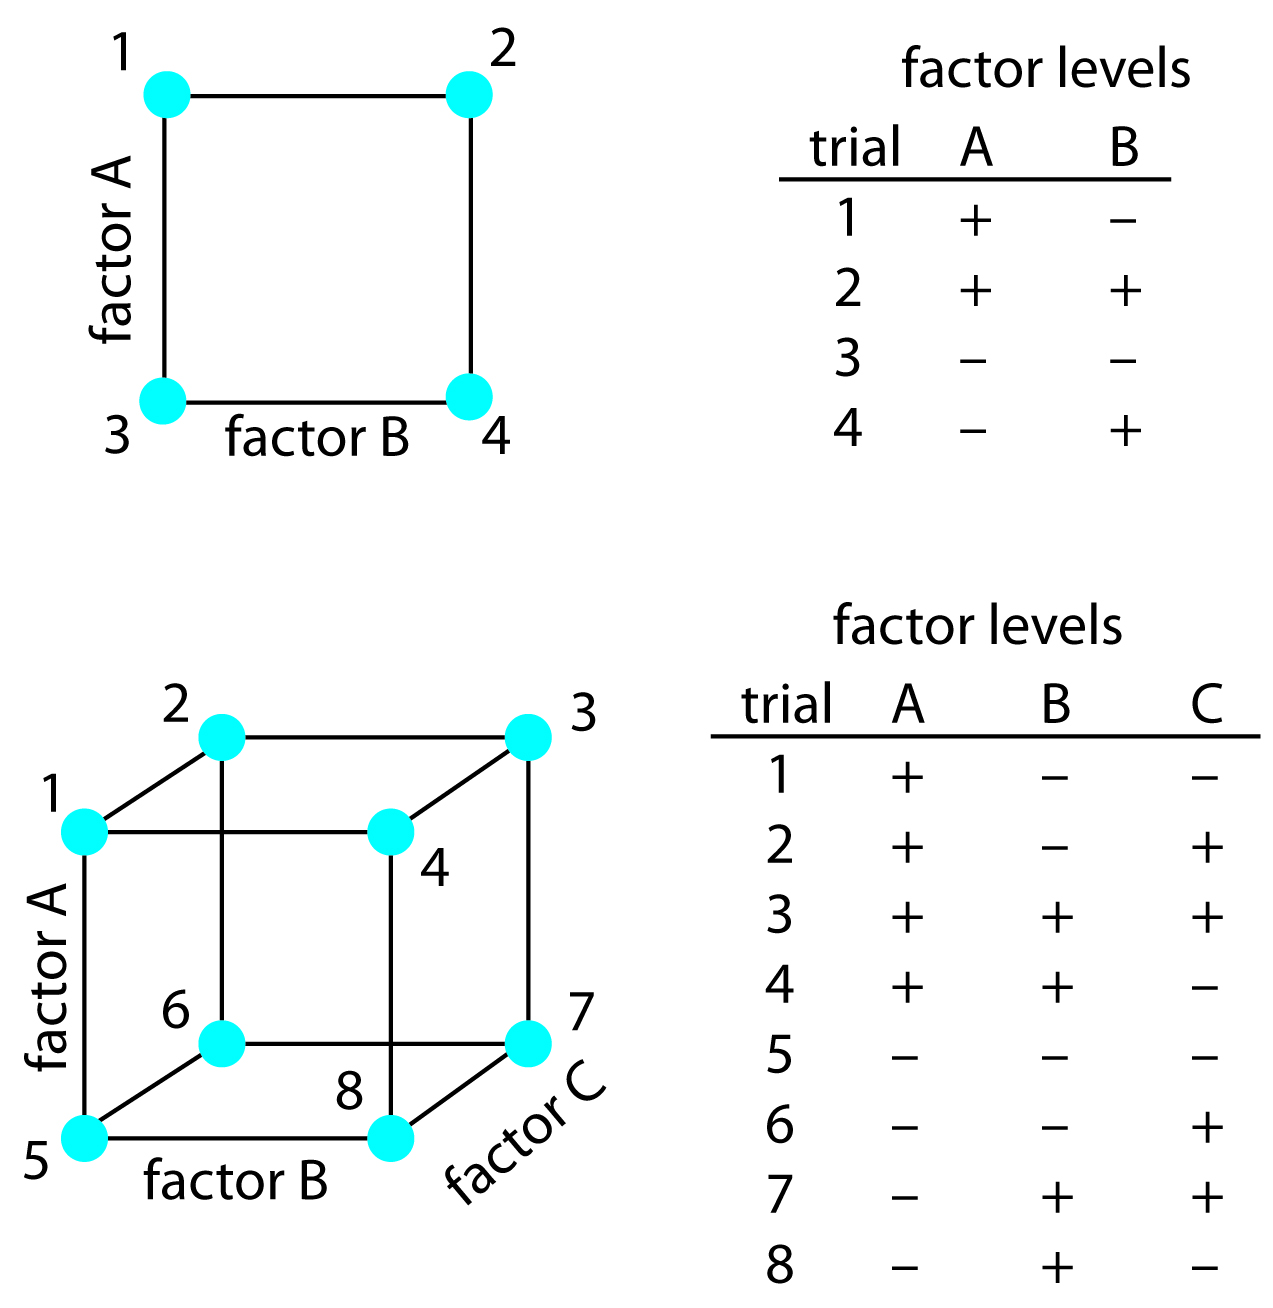
\includegraphics[width=0.7\linewidth, height=0.3\textheight]{art/full_factorial}
\caption{Full factorial designs: $2^2$ and $2^3$. \newline \url{http://chemwiki.ucdavis.edu/Analytical_Chemistry/Analytical_Chemistry_2.0/14_Developing_a_Standard_Method}}
\label{fig:full_factorial}
\end{figure}
With this $2^2$ design, we may recover several effects:
The effect of varying $A$ from $-$ to $+$: the \emph{main effect of $A$} typically denoted $a$. 
The effect of varying $B$ from $-$ to $+$: the \emph{main effect of $B$} typically denoted $b$.  
The effect of varying both $A$ and $B$ from $-$ to $+$. 
We denote the expected response at $A=-,B=-$ with $\mu_{--}$, and the other conditions respectively.
We denote $ab=\mu_{++}-\mu_{--}-a-b$.
If $ab=0$ we say there is \emph{no interaction}.
If $ab \neq 0$, it means that the effect of $A$ depends on the state of $B$, or conversely, that the effect of $B$ depends on the state of $A$.  In short, if $ab \neq 0$ we say there is an \emph{interaction} between $A$ and $B$. \marginnote{Interaction}

Slightly intruding into the realm of data analysis, a visualization of interactions is known as the \emph{interaction plot}, depicted in Figure~\ref{fig:interaction_plot}. 
The upper left panel demonstrates a lack of interaction (think why), while the upper right panel depicts an interaction.
\begin{figure}[ht]
\centering
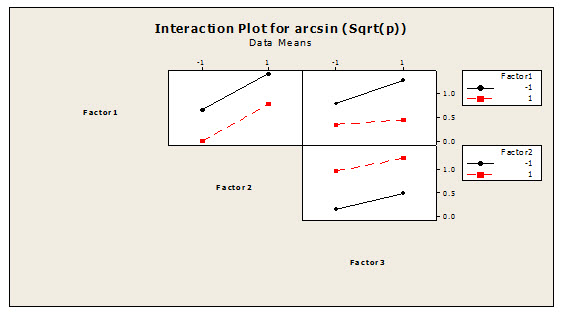
\includegraphics[width=0.3\textheight]{art/attribute_doe_interaction_plot}
\caption{Interactions plot. \newline \url{http://blog.minitab.com/blog/statistics-in-the-field/optimizing-attribute-responses-using-design-of-experiments-doe-part-2}}
\label{fig:interaction_plot}
\end{figure}



\begin{remark}[Intermediate Factor Levels]
In a $2^k$ design, a factor may actually be a continuous controllable input which was restricted to two values for convenience. 
After estimating the effect of the factor, we may want to know what would the effect have been, were we to set it on some intermediate level.
It is customary to assume that a main effect acts linearly in-between experimental conditions, yet you should remember that there is nothing in the data to support this.
For a more rigorous approach, see the Response Surface Methodology section (\ref{sec:response_surface}).
\end{remark}



\subsubsection{$3^k$ Designs}
I think that the name $3^k$ design is rather self explanatory.
Then again, more than $2$ levels are rarely treated as factorial experiments, but rather in the Response Surface methodology of Section~\ref{sec:response_surface}.




\subsection{Fractional Factorial}
The full factorial designs are the simplest designs to setup and interpret. 
A major drawback, are the resources required when $k$ is large. 
This is where the \emph{fractional factorial}, or \emph{partial factorial} designs kick in.
The fundamental idea is to design a full factorial, but skip a couple experimental conditions. 

\begin{example}[From $2^2$ to $2^{(2-1)}$]
\label{eg:fractional_factorial}
As a first example, we will try to save some time and money by eliminating particular conditions of the $2^2$ design in Figure~\ref{fig:full_factorial}.
As the name may suggest, a $2^{2-1}$ design, has $2$ experimental conditions in each run. 
There are thus $\binom{4}{2}=6$ possible eliminations.
\begin{table}
\begin{tabular}{|p{2.5cm}|p{10cm}|}
\hline Elimination &  Problem \\ 
\hline
\hline 1,2 &  No information on $a$. \\ 
\hline 1,3 &  No information on $b$.\\ 
\hline 1,4 &  $a$ aliased with $b$ aliased with $ab$. \\ 
\hline 2,3 &  $a$ aliased with $b$ aliased with $ab$. \\ 
\hline 2,4 &  No information on $b$. \\ 
\hline 3,4 &  No information on $a$.\\ 
\hline 
\end{tabular} 
\label{tab:partial_factorial}
\caption{$2^{2-1}$: All possible eliminations from the $2^2$ design that lead to a $2^{2-1}$ design.}
\end{table}
\end{example}

The lesson from Example~\ref{eg:fractional_factorial} is that in a fractional factorial our savings in time and money, come at the cost of the information that can be drawn from the experiment.
The idea behind partial factorial experiments, is that by an informed choice of the conditions skipped, we can choose what information to give up.




\subsubsection{Confounding of Effects}

\subsubsection{Design Resolution}


\subsection{Screening Experiments}

\section{Random Effects}

\subsection{Randomized Block Designs}

\subsubsection{Complete Block Designs}


\subsubsection{Latin Square Design}

\subsubsection{Latin Square Design}

\subsubsection{Cross Over Design}

\subsubsection{Incomplete Block Designs}


\subsection{Random Effects Factors}

\subsection{Nested Designs}


\subsubsection{Nested and Crossed Designs}

\subsubsection{Split Plot Designs}




\subsection{Process Improvement Designs}



\subsubsection{Taguchi's Robust Design Approach}



\section{Continuous Factors}



\subsection{Response Surface Methdology}
\label{sec:response_surface}

\subsubsection{Central Composite Design}

\subsubsection{Box-Behnken Design}

\subsection{Optimal Designs}

\subsubsection{A optimality}
\subsubsection{B optimality}
\subsubsection{C optimality}
\subsubsection{D optimality}




\section{Sequential Designs}
% Mark Vandelmeulenbruke

\subsubsection{Active Learning}


\subsubsection{MultiArmed Bandits}




\section{Adaptive Designs}



\section{Computer Experiments}

